\documentclass[10pt,twocolumn]{article}

% --- Page and font ---
\usepackage[letterpaper,margin=0.50in]{geometry}
\usepackage{mathpazo}
\usepackage[T1]{fontenc}
\usepackage{microtype}
\usepackage{amsmath,amssymb}
\usepackage{xcolor}
\usepackage{tikz}
\usepackage{graphicx}
\usetikzlibrary{arrows.meta,positioning,calc,fit,shapes.geometric}
\usepackage{titlesec}
\usepackage{caption}
\usepackage{enumitem}
\usepackage{tcolorbox}
\usepackage[colorlinks=true,linkcolor=deepblue,citecolor=deepblue,urlcolor=deepblue]{hyperref}

% --- Muted palette, close to the uploaded page ---
\definecolor{deepblue}{RGB}{59,76,95}
\definecolor{lineblue}{RGB}{83,103,122}
\definecolor{softblue}{RGB}{235,242,247}
\definecolor{cellblue}{RGB}{221,232,238}
\definecolor{cellgreen}{RGB}{226,237,229}
\definecolor{cellgray}{RGB}{238,239,239}
\definecolor{mutedred}{RGB}{155,54,62}
\definecolor{mutedteal}{RGB}{55,115,120}

% --- Compact readable layout ---
\setlength{\columnsep}{0.28in}
\setlength{\parindent}{0pt}
\setlength{\parskip}{1.0pt}
\setlength{\textfloatsep}{3pt plus 1pt minus 1pt}
\setlength{\floatsep}{3pt plus 1pt minus 1pt}
\setlength{\intextsep}{3pt plus 1pt minus 1pt}
\captionsetup{font=scriptsize,labelfont=bf,skip=1pt}
\titleformat{\section}{\normalsize\bfseries\color{deepblue}}{\thesection}{0.45em}{}
\titlespacing*{\section}{0pt}{3.5pt}{1pt}
\renewcommand{\thesection}{\Alph{section}}
\pagestyle{plain}

\tcbset{
  cvtbox/.style={
    colback=softblue,
    colframe=lineblue,
    boxrule=0.45pt,
    arc=2pt,
    left=3pt,right=3pt,top=3pt,bottom=3pt,
    before skip=2pt,after skip=2pt
  }
}

\begin{document}

\appendix
\twocolumn[{
\begin{center}
{\LARGE\bfseries\color{deepblue} Appendix B: Centroidal Voronoi Tessellations}\\[-0.2ex]
\end{center}
}]

\section{Representative Placement}
Imagine placing $k$ hospitals to cover a city. A natural assignment rule sends each neighbourhood to the nearest hospital, while a natural placement rule asks each hospital to lie near the centre of the area it serves. When these two requirements are satisfied simultaneously, the resulting structure is a \textbf{Centroidal Voronoi Tessellation} (CVT).

This concept, formalised by Du, Faber, and Gunzburger~\cite{du1999cvt}, appears in image compression, mesh generation, clustering, and optimal quantisation. Here, CVTs divide the compression configuration space into balanced and well-separated search regions, each maintained as an independent population in the genetic search. The construction rests on two notions: Voronoi cells and centroids.

\section{Voronoi Assignment}
Let $\Omega$ be a bounded region and let $\{z_i\}_{i=1}^k$ be a set of chosen points inside it. These points are the \textbf{generators}. The Voronoi cell $V_i$ associated with generator $z_i$ contains exactly the points of $\Omega$ for which $z_i$ is the nearest generator~\cite{mount2002geom}:
\begin{tcolorbox}[cvtbox]
\[
V_i=\{x\in\Omega\mid \lVert x-z_i\rVert < \lVert x-z_j\rVert,\ \forall j\ne i\}.
\]
\end{tcolorbox}
The cells $\{V_i\}$ tile $\Omega$ without gaps or overlaps. Their boundaries are perpendicular bisectors between neighbouring generator pairs. In the genetic search, this gives each compression configuration a unique region assignment and avoids ambiguity between populations.

\begin{figure}[ht]
\centering
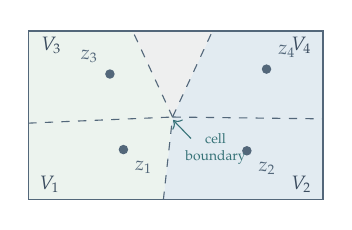
\begin{tikzpicture}[scale=0.78, every node/.style={font=\scriptsize}]
  \coordinate (A) at (0,0); \coordinate (B) at (4.8,0); \coordinate (C) at (4.8,2.75); \coordinate (D) at (0,2.75);
  \coordinate (P) at (2.35,1.35);
  \fill[cellgreen!65] (A)--(2.2,0)--(P)--(1.7,2.75)--(D)--cycle;
  \fill[cellblue!85] (2.2,0)--(B)--(C)--(3.0,2.75)--(P)--cycle;
  \fill[cellgray] (1.7,2.75)--(3.0,2.75)--(P)--cycle;
  \fill[cellblue!55] (A)--(B)--(2.2,0)--cycle;
  \draw[lineblue,thin] (A) rectangle (C);
  \draw[lineblue,dashed] (2.2,0)--(P)--(1.7,2.75);
  \draw[lineblue,dashed] (P)--(3.0,2.75);
  \draw[lineblue,dashed] (P)--(4.8,1.32);
  \draw[lineblue,dashed] (0,1.25)--(P);
  \fill[lineblue] (1.55,0.82) circle (2.2pt) node[below right=1pt] {$z_1$};
  \fill[lineblue] (3.56,0.80) circle (2.2pt) node[below right=1pt] {$z_2$};
  \fill[lineblue] (1.33,2.05) circle (2.2pt) node[above left=1pt] {$z_3$};
  \fill[lineblue] (3.88,2.13) circle (2.2pt) node[above right=1pt] {$z_4$};
  \node[deepblue] at (0.35,0.25) {$V_1$};
  \node[deepblue] at (4.45,0.25) {$V_2$};
  \node[deepblue] at (0.38,2.52) {$V_3$};
  \node[deepblue] at (4.45,2.52) {$V_4$};
  \draw[mutedteal,->,thin] (2.65,1.00) -- (2.36,1.30);
  \node[mutedteal,align=center,font=\tiny] at (3.05,0.83) {cell\\boundary};
\end{tikzpicture}
\caption{Voronoi diagram with four generators. Each region $V_i$ contains the points closest to its generator.}
\end{figure}

\section{Density-Weighted Centroids}
The \textbf{centroid} of a region is its density-weighted average position. For a region $V$ with density function $\rho$, it is defined as
\[
 z^{\ast}=\frac{\int_V y\,\rho(y)\,dy}{\int_V \rho(y)\,dy}.
\]
For a uniform rectangle, the centroid is the geometric centre. For an irregular region or non-uniform density, it shifts toward the side carrying more mass.

A generator $z_i$ placed arbitrarily in $\Omega$ does not generally coincide with the centroid $z_i^{\ast}$ of its Voronoi cell. The generator defines the cell, whereas the centroid is computed after the assignment has been made.

\section{Centroidal Consistency}
A \textbf{Centroidal Voronoi Tessellation} is a Voronoi diagram in which every generator is also the centroid of its associated cell~\cite{du1999cvt}:
\begin{tcolorbox}[cvtbox]
\[
 z_i=z_i^{\ast}\quad \forall i, \qquad \text{i.e., generator = centroid of its cell.}
\]
\end{tcolorbox}
This condition couples assignment and placement. Moving a generator changes the Voronoi boundaries, which changes the centroids and may require further generator updates. A CVT is a fixed point of this process. In the genetic search, it gives stabilised regions whose representatives lie at the centres of their assigned territories. Figure~\ref{fig:cvtcompare} illustrates this condition.


\begin{figure}[ht]
\centering
\resizebox{0.995\linewidth}{!}{%
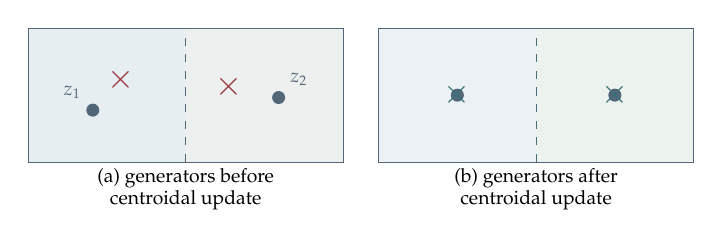
\begin{tikzpicture}[every node/.style={font=\scriptsize}]
  % non-centroidal Voronoi assignment
  \begin{scope}
    \fill[cellblue!75] (0,0) rectangle (4.00,1.70);
    \fill[cellgray] (2.00,0) rectangle (4.00,1.70);
    \draw[lineblue,thin] (0,0) rectangle (4.00,1.70);
    \draw[lineblue,dashed] (2.00,0)--(2.00,1.70);
    \fill[lineblue] (0.82,0.66) circle (2.35pt) node[above left=1pt] {$z_1$};
    \fill[lineblue] (3.18,0.82) circle (2.35pt) node[above right=1pt] {$z_2$};
    \node[mutedred,font=\large] at (1.18,1.05) {$\times$};
    \node[mutedred,font=\large] at (2.55,0.95) {$\times$};
    \node[align=center,font=\scriptsize] at (2.00,-0.34) {(a) generators before\\centroidal update};
  \end{scope}
  % centroidal Voronoi assignment
  \begin{scope}[xshift=4.45cm]
    \fill[cellblue!60] (0,0) rectangle (2.00,1.70);
    \fill[cellgreen!65] (2.00,0) rectangle (4.00,1.70);
    \draw[lineblue,thin] (0,0) rectangle (4.00,1.70);
    \draw[lineblue,dashed] (2.00,0)--(2.00,1.70);
    \fill[lineblue] (1.00,0.85) circle (2.35pt);
    \node[mutedteal,font=\large] at (1.00,0.85) {$\times$};
    \fill[lineblue] (3.00,0.85) circle (2.35pt);
    \node[mutedteal,font=\large] at (3.00,0.85) {$\times$};
    \node[align=center,font=\scriptsize] at (2.00,-0.34) {(b) generators after\\centroidal update};
  \end{scope}
\end{tikzpicture}%
}
\caption{The centroidal condition aligns each generator with the centroid of its assigned Voronoi cell.}
\label{fig:cvtcompare}
\end{figure}

\section{Lloyd Iteration}
A standard construction procedure is \textbf{Lloyd's algorithm}~\cite{du1999cvt}, which alternates between nearest-generator assignment and centroidal relocation:
\begin{enumerate}[leftmargin=1.15em,itemsep=0pt,topsep=1pt]
\item Initialise $k$ generators at random positions in $\Omega$.
\item Build the Voronoi diagram by assigning each point or sample to its nearest generator.
\item Move every generator to the centroid of its current cell.
\item Repeat the assignment and relocation steps until the generators no longer move appreciably.
\end{enumerate}

\section{Energy Formulation of CVTs}
The CVT condition also has an energy formulation. For a partition $\{V_i\}_{i=1}^k$ and generators $\{z_i\}_{i=1}^k$, define the \textbf{quantisation error}, also called total inertia, as~\cite{du1999cvt}
\[
 \mathcal{E}=\sum_{i=1}^{k}\int_{V_i}\rho(y)\,\lVert y-z_i\rVert^2\,dy.
\]
This objective measures the density-weighted squared distance from points in $\Omega$ to their assigned generators. Minimising $\mathcal{E}$ over the partition gives the Voronoi assignment rule; minimising it over the generator locations places each generator at the centroid of its cell. The stationary structure therefore satisfies the CVT condition.

\begin{tcolorbox}[cvtbox]
\textbf{Energy interpretation.} Lloyd's algorithm can be viewed as alternating minimisation of $\mathcal{E}$. With fixed generators, the nearest-generator Voronoi assignment minimises the distance term. With fixed cells, replacing each generator by the corresponding centroid minimises the same objective inside that cell. The resulting compact regions help the genetic search maintain distinct populations over different parts of the compression configuration space.
\end{tcolorbox}

\begingroup\scriptsize
\setlength{\itemsep}{0pt}
\setlength{\parskip}{0pt}
\begin{thebibliography}{9}
\bibitem{du1999cvt}
Q. Du, V. Faber, and M. Gunzburger. \textit{Centroidal Voronoi Tessellations: Applications and Algorithms}. SIAM Review, 41(4):637--676, 1999.
\bibitem{mount2002geom}
D. M. Mount. \textit{CMSC 754 Computational Geometry Lecture Notes}. University of Maryland, 2002.
\end{thebibliography}
\endgroup

\end{document}
